\documentclass[review,11pt]{elsarticle}

\usepackage[T1]{fontenc}
\usepackage{amsmath,amssymb}
\usepackage{booktabs}
\usepackage{graphicx}
\usepackage{xcolor}
\usepackage{multirow}
\usepackage{hyperref}

\newcommand{\todo}[1]{\textcolor{red}{[TODO: #1]}}
\newcommand{\RE}{\mathrm{RE}}

\journal{Applied Soft Computing}

\begin{document}

\begin{frontmatter}

\title{Genetic Programming Hyper-Heuristics for the Job Shop Scheduling
Problem with Interval Durations: Interpretable Rules that Generalize
Across Instance Sizes}

\author{Hern\'an D\'iaz}
\affiliation{organization={Department of Computer Science, University of Oviedo},
            city={Gij\'on},
            country={Spain}}

\begin{abstract}
Dispatching rules remain the method of choice for scheduling under tight
time budgets, but hand-crafted rules leave substantial performance
unexploited, and the automated design of rules has scarcely been explored
for scheduling problems with non-deterministic processing times. We present
a genetic programming (GP) hyper-heuristic for the job shop scheduling
problem with interval durations (IJSP), in which operation durations are
known only to lie within an interval and schedules are evaluated by
interval arithmetic. The GP evolves priority expressions over an
\emph{interval-aware} terminal set that exposes both the worst-case values
and the widths of the uncertain quantities, so that evolved rules can react
to uncertainty itself. On the 70 interval versions of Taillard's benchmark,
over 30 independent evolutions the resulting rules average a relative
error of $18.7\%$ ($\pm0.8$) with a single deterministic constructive
pass, and the best evolved rule attains $17.3\%$---improving on the
strongest deterministic constructive baseline (Giffler--Thompson with MWKR
tie-breaking, $29.5\%$) on every single instance---and generalizes
zero-shot across all seven instance size classes despite being evolved on
only four training instances of a single size class ($20{\times}15$).
Embedded in a GRASP-style randomized scheme, the evolved rule
converts sampling budget into solution quality ($13.7\%$ at best-of-1024).
Evolved rules are compact, human-readable expressions, and an automatic
configuration study with irace shows the approach is robust to its own
hyperparameters, with a preference for \emph{smaller} expression trees at
no performance cost. We position the method against fixed rules, active
schedule generators, and published metaheuristics, characterizing the
computational class in which interpretable evolved rules operate.
\end{abstract}

\begin{keyword}
interval job shop scheduling \sep genetic programming \sep hyper-heuristics
\sep dispatching rules \sep scheduling under uncertainty \sep robustness
\end{keyword}

\end{frontmatter}

\section{Introduction}
\label{sec:intro}

Real manufacturing environments rarely know the exact duration of an
operation in advance. The interval job shop scheduling problem (IJSP)
models this uncertainty in a minimal, distribution-free way: each
processing time is only assumed to lie within a known interval, schedules
are built and evaluated with interval arithmetic, and solutions are
compared by their worst-case (upper-bound) makespan. Population
metaheuristics for the IJSP---artificial bee colony variants and tabu
search among them---achieve strong results at the cost of minutes of
per-instance search~\cite{DiazFEABC2023,DiazICAE2023,DiazTS2026}.

At the opposite end of the computational spectrum live \emph{dispatching
rules}: priority functions that build a schedule in a single constructive
pass by repeatedly selecting the next operation to start. Their appeal is
threefold---speed, interpretability, and trivial deployment---but
hand-crafted rules (SPT, MOR, MWKR and relatives) leave a large quality
gap: on the benchmark used in this paper the best fixed rule averages
$45.5\%$ relative error, versus $4$--$10\%$ for metaheuristics.

For \emph{deterministic} scheduling, a rich literature has shown that this
gap can be narrowed substantially by evolving rules automatically with
genetic programming (GP)~\cite{Branke2016,Nguyen2017}. For scheduling
under interval uncertainty, however, the automated design of dispatching
rules remains, to the best of our knowledge, unexplored. It is not obvious
a priori what an evolved rule should do with uncertainty: ignore it and
rank by worst case, hedge against wide intervals, or exploit width
information in a structured way. Making this possible requires exposing
uncertainty to the rule as first-class attributes.

This paper makes the following contributions:
\begin{enumerate}
\item A GP hyper-heuristic for the IJSP whose terminal set is
  \emph{interval-aware}: alongside worst-case processing time, earliest
  start and work remaining, rules can read the \emph{widths} of these
  quantities, enabling uncertainty-sensitive prioritization
  (Section~\ref{sec:method}).
\item An empirical study on the 70 interval Taillard instances showing
  that evolved rules (i) beat every deterministic constructive baseline by
  a wide margin at equal cost, (ii) generalize zero-shot across instance
  sizes---evolved on $20{\times}15$, best class $50{\times}15$---and
  (iii) extend naturally to a randomized multi-start regime with monotone
  quality gains up to best-of-1024 (Section~\ref{sec:results}).
\item An analysis of \emph{why} the rules work: an anatomy of the evolved
  expressions (Section~\ref{sec:anatomy}), an ablation isolating the
  contribution of the interval-width terminals
  (Section~\ref{sec:ablation}), and an executional-robustness study showing
  that the evolved rule yields schedules whose realized makespan deviates
  less from its prediction than the baselines', increasingly so as
  uncertainty grows (Section~\ref{sec:robustness}).
\item An automatic configuration study (irace, 200 experiments) of the
  evolutionary hyperparameters, confirmed over 30 independent evolutions
  per configuration: tuning brings no significant quality gain---the
  method is robust to its own knobs---but does yield systematically
  smaller, more readable trees at equal performance
  (Section~\ref{sec:tuning}).
\end{enumerate}

The remainder of the paper is organized as follows.
Section~\ref{sec:related} reviews related work.
Section~\ref{sec:problem} formalizes the IJSP.
Section~\ref{sec:method} presents the GP hyper-heuristic and its
interval-aware terminal set. Section~\ref{sec:setup} details the
experimental protocol, and Section~\ref{sec:results} the empirical study,
including the hyperparameter analysis. Section~\ref{sec:conclusions}
concludes.

\section{Related Work}
\label{sec:related}

\subsection{Job shop scheduling under interval uncertainty}
Interval durations offer a distribution-free uncertainty model requiring
only bounds, in contrast to stochastic and fuzzy
approaches~\cite{FuzzyJSPRef}. Prior IJSP work is dominated by
population-based metaheuristics: a genetic algorithm with a systematic
study of interval rankings~\cite{DiazGA2020}, artificial bee colony
variants~\cite{DiazFEABC2023,DiazICAE2023}, and a population-based tabu
search that currently defines the state of the art~\cite{DiazTS2026}. All operate in
the minutes-per-instance regime. Fast constructive methods for the IJSP
have received far less attention; dispatching rules with interval-aware
lexicographic comparisons are the de facto baseline.

\subsection{Automated design of dispatching rules}
GP hyper-heuristics evolve priority expressions over scheduling
attributes, and constitute the standard approach to automated rule design
for production scheduling~\cite{Branke2016,Nguyen2017}. Evolved rules
have been shown to outperform hand-crafted ones across job shop variants,
with active research on surrogate fitness, feature selection, and
multi-objective formulations. Beyond single rules, a productive line
combines several evolved rules into \emph{ensembles} that jointly
construct or vote on a solution~\cite{GilGala2021Ensembles}, and recent
work explores alternatives to evolutionary search for the same design
task---systematic tree search over the space of expression
trees~\cite{GilGala2025SSHE}---reporting rules of comparable quality but
smaller size and better readability. All of this work targets
deterministic (or dynamic-stochastic) settings. Closest to our setting,
Karunakaran et
al.~\cite{Karunakaran2017} evolve rules for dynamic job shops with
uncertain processing times, exposing summary statistics of observed
deviations (an exponential moving average) to the rule; uncertainty there
is realized stochastically during simulation, and rules are evaluated on
sampled scenarios. A recent survey of learned optimisation for the job
shop~\cite{Xu2025}, covering both GP and DRL constructive approaches,
records no work on interval-valued processing times. To the best of our
knowledge, evolving rules whose \emph{inputs} are interval
attributes---and whose fitness is computed by interval arithmetic rather
than by sampling realizations---has not been explored before.

\subsection{Learned constructive heuristics}
Deep reinforcement learning provides an alternative family of learned
constructive methods for the JSP~\cite{Zhang2020L2D,Park2021GNN}; GP
rules and DRL policies are increasingly studied as competing
learning paradigms for the same construction task, and controlled
comparisons between them under common protocols have been identified as
a gap in the recent literature~\cite{Xu2025}. Both families occupy the
same computational class at deployment (a single constructive pass); a
controlled comparison on the IJSP is beyond the scope of this paper and
is the object of ongoing work.

\section{The Interval Job Shop Scheduling Problem}
\label{sec:problem}

An IJSP instance consists of $n$ jobs and $m$ machines. Job $j$ is a
chain of $m$ operations $o_{j1} \prec o_{j2} \prec \cdots \prec o_{jm}$,
each requiring a distinct machine $\mu(o_{jk})$ exclusively and
non-preemptively. The duration of operation $o$ is an interval
$p_o = [\underline{p}_o, \overline{p}_o]$ with
$0 < \underline{p}_o \le \overline{p}_o$: the only assumption is that the
realized duration lies within these bounds.

Schedule construction uses interval arithmetic. For intervals
$a=[\underline{a},\overline{a}]$ and $b=[\underline{b},\overline{b}]$:
$a + b = [\underline{a}+\underline{b},\, \overline{a}+\overline{b}]$ and
$\max(a,b) = [\max(\underline{a},\underline{b}),\,
\max(\overline{a},\overline{b})]$ (component-wise). Given an operation
processing order (a permutation with repetition of jobs, decoded left to
right), the \emph{semiactive} schedule starts each operation at
$s_o = \max(C_{\mathrm{job}}, C_{\mathrm{mach}})$---the component-wise
maximum of the completion intervals of its job predecessor and machine
predecessor---and completes at $C_o = s_o + p_o$. The makespan
$C_{\max} = \max_j C_{o_{jm}}$ (component-wise maximum) is itself an
interval. Since intervals admit no natural total order, schedules are
compared with an interval ranking: we use the lexicographic order
$\leq_{Lex2}$ (upper bound first, lower bound as tie-break), one of the
standard rankings of the IJSP literature and the one found
in~\cite{DiazGA2020} to yield the most robust schedules; the midpoint
ranking $\leq_{MP}$---equivalent to the possibility-degree method
of~\cite{Lei2012}---underlies the $E[C_{\max}]$ metric in which results
are reported. All methods in this
paper---the GP rules and every baseline---share one implementation of
this decoder and evaluator, so reported differences cannot stem from
evaluator discrepancies.

Performance is reported as relative error against the crisp Taillard
lower bounds: $\RE = (E[C_{\max}] - LB)/LB \times 100$, where
$E[C_{\max}]$ is the midpoint of the interval makespan.

\section{GP Hyper-Heuristic for the IJSP}
\label{sec:method}

\subsection{Rule representation}
An individual is a priority expression tree. Leaves are drawn from the
interval-aware terminal set of Table~\ref{tab:terminals}; internal nodes
from $\{+, -, \times, \div_p, \min, \max, \mathrm{neg}\}$ with protected
division. At each scheduling decision the tree is evaluated (vectorized)
over all eligible operations and the operation with \emph{lowest}
priority is dispatched, yielding a semiactive schedule. Classic rules are
points of this search space---SPT is the tree $\mathit{PT}$ and MWKR is
$\mathrm{neg}(\mathit{WKR})$---and both are injected as seed individuals.

\begin{table}[t]
\centering\small
\caption{Interval-aware terminal set, with exact definitions. For an
eligible operation $o$ of job $j$ on machine $m$: $p_o =
[\underline{p}_o, \overline{p}_o]$ is its duration interval; $C_j$ and
$C_m$ are the (interval) completion times of the last scheduled operation
of job $j$ and machine $m$; $\mathcal{R}_o$ is the set of operations of
$j$ after $o$; $\mathcal{E}$ is the current eligible set. Terminals are
evaluated on \emph{raw} (unnormalized) values.}
\label{tab:terminals}
\begin{tabular}{lll}
\toprule
Terminal & Definition & Role \\
\midrule
PT   & $\overline{p}_o$ & worst-case processing time \\
PTW  & $\overline{p}_o-\underline{p}_o$ & duration uncertainty \\
EST  & $\overline{e}_o = \max(\overline{C}_j, \overline{C}_m)$ &
worst-case earliest start \\
ESTW & $\overline{e}_o - \underline{e}_o$, with
$\underline{e}_o=\max(\underline{C}_j,\underline{C}_m)$ &
start uncertainty \\
WKR  & $\sum_{q\in\mathcal{R}_o}\overline{p}_q$ & worst-case work
remaining \\
WKRW & $\sum_{q\in\mathcal{R}_o}(\overline{p}_q-\underline{p}_q)$ &
remaining-work uncertainty \\
NOR  & $|\mathcal{R}_o|$ & operations remaining \\
SLACK& $\overline{e}_o - \min_{o'\in\mathcal{E}}\overline{e}_{o'}$ &
start slack within eligible set \\
ONE  & $1$ & constant \\
\bottomrule
\end{tabular}
\end{table}

Protected division is defined as $a \div_p b = a/b$ if $|b| > 10^{-9}$
and $a$ otherwise. Priority ties at dispatch time are broken by eligible
set order (lowest job index first), which is deterministic; hence a rule
maps each instance to exactly one schedule.

\subsection{Evolution}
Generational GP with the operators and parameters of
Table~\ref{tab:gpparams}. Initialization is ramped half-and-half over
depths $2$--$4$ (grow trees terminate early with probability $0.3$ per
node), with SPT and MWKR injected as two additional seed individuals.
Each generation, the elite passes unchanged and the remainder is produced
by tournament selection followed by subtree crossover (a uniformly random
node of parent A is replaced by a uniformly random subtree of parent B)
or, with the complementary probability, subtree mutation (a uniformly
random node is replaced by a fresh grow tree of depth $\le 3$). Offspring
exceeding the node cap receive fitness $\infty$ (bloat control). Fitness
of a rule is the mean $\RE$ of its deterministic rollout over the four
training instances---computed with the same environment, decoder and
evaluator used by all baselines, which eliminates evaluator mismatch as
a confound.

\begin{table}[t]
\centering\small
\caption{Evolution parameters (conventional settings; see
Section~\ref{sec:tuning} for the sensitivity study).}
\label{tab:gpparams}
\begin{tabular}{ll}
\toprule
Population / generations & $100$ / $50$ \\
Initialization & ramped half-and-half, depths $2$--$4$ + \{SPT, MWKR\} \\
Selection & tournament, size $4$ \\
Crossover / mutation prob. & $0.8$ / $0.2$ (subtree; mutation depth $\le 3$) \\
Elitism & $2$ \\
Tree-size cap & $40$ nodes (violations: fitness $\infty$) \\
Fitness & mean RE, deterministic rollout, TA11--TA14 \\
Seeds & $1$--$30$ (RNG of evolution and environment) \\
\bottomrule
\end{tabular}
\end{table}

\subsection{Randomized multi-start extension}
A deterministic rule produces one schedule. For matched comparisons with
sampling-based methods we wrap the evolved rule in GRASP-style
randomization: with probability $\varepsilon{=}0.1$ the dispatched
operation is drawn uniformly from the eligible set, otherwise the rule
decides; sample $0$ remains deterministic. Best-of-$N$ then reports the
lexicographically best schedule. This uniform perturbation of a single
rule is the simplest member of a broader family of randomized rule-based
builders; a richer alternative, orthogonal to our contribution, swaps
among a \emph{set} of evolved rules during
construction~\cite{GilGala2025GRASB}.

\section{Experimental Setup}
\label{sec:setup}

\textbf{Instances.} The 70 interval versions of Taillard's instances
(TA1--TA70, seven size classes from $15{\times}15$ to $50{\times}20$),
with crisp Taillard lower bounds as the $\RE$ reference. Each interval
instance is derived from its crisp counterpart with the generation scheme
introduced in~\cite{DiazGA2020}: every duration $p$ is replaced by the
integer interval $[p-\delta,\, p+\delta]$, with $\delta$ drawn uniformly
in $[0,\, 0.15\,p]$ (maximum deviation $15\%$); machine routes are
unchanged. The midpoint of every interval thus equals the original
duration---the crisp instance is exactly the midpoint scenario of its
interval version---which makes the crisp Taillard bounds a meaningful
reference for $E[C_{\max}]$. After integer rounding, ${\approx}20\%$ of
operations end up degenerate (deterministic), and the mean relative width
is ${\approx}13\%$. The same scheme underlies the benchmark of the
published IJSP
metaheuristics~\cite{DiazGA2020,DiazFEABC2023,DiazICAE2023}, and the
interval Taillard set is the one used in~\cite{DiazTS2026}, which makes
the comparison against those methods an exact one (identical uncertainty
model and benchmark).

\textbf{Data split and exclusions.} Rules are evolved on TA11--TA14
($20{\times}15$), and TA15--TA20 serve as development set: they never contribute to fitness,
but design and configuration decisions (including the irace study of
Section~\ref{sec:tuning}) were selected on their performance, so we flag
them as subject to development reuse. The remaining 60 instances are
fully unseen by every design decision and constitute the honest
generalization test.

\textbf{Budgets.} Population $100$, $50$ generations: ${\sim}20{,}400$
fitness rollouts (${\approx}30$ min single-core) per seed; thirty
independent seeds per configuration, following standard practice in
evolutionary computation.

\textbf{Baselines.} Fixed rules (SPT, LPT, MOR, MWKR) with interval-aware
lexicographic comparison; the Giffler--Thompson active-schedule generator
with rule tie-breaks (deterministic and $\varepsilon$-randomized inside
the conflict set); published IJSP metaheuristics
(fEABC~\cite{DiazFEABC2023}, ESABC~\cite{DiazICAE2023},
TS~\cite{DiazTS2026}) as yardsticks of the search-based computational
class.

\section{Results}
\label{sec:results}

\subsection{Evolution behaviour and seed stability}
Over 30 independent evolutions, training $\RE$ converges to
$14.8 \pm 0.9$ (range $13.4$--$16.9$), with most of the improvement
realized by generation $25$--$30$ (Figure~\ref{fig:convergence}). The
evolved rules are structurally recognizable, combining the classical
dispatching ingredients in interpretable ways. The best rule of the
campaign (seed~27), for instance, is built from the ratio
$\mathit{SLACK}/\mathit{PT}$ (slack per unit of processing time), work
remaining terms bounded by operations-remaining counts, and an
earliest-start correction---a refinement of the
most-work-remaining/earliest-start family that hand-crafted rules
approximate only coarsely.

\begin{figure}[t]
\centering
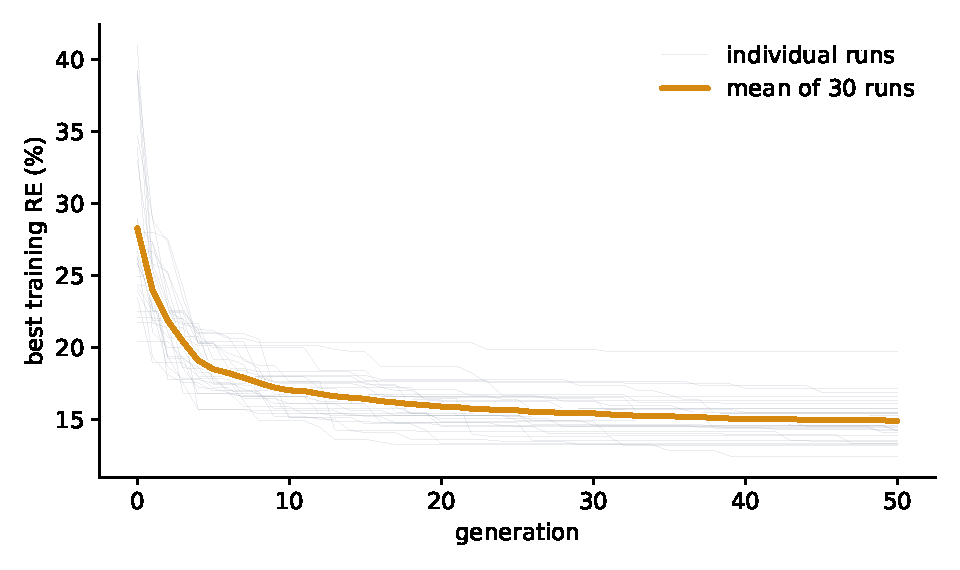
\includegraphics[width=.8\linewidth]{figures/fig_convergence.pdf}
\caption{Best training fitness per generation for the 30 evolution seeds
(default configuration): individual runs (grey) and their mean (amber).}
\label{fig:convergence}
\end{figure}

\subsection{Rule anatomy and interpretability}
\label{sec:anatomy}
A practical appeal of GP over neural policies is that its output is a
readable expression. Evolved rules are compact---mean tree size $33$
nodes ($19$--$40$), mean depth $10$---so a rule can be inspected
and simplified by hand. Figure~\ref{fig:terminals} reports how often each
terminal is used across the 30 evolved rules. The backbone is the
classical scheduling triad---slack (\textit{SLACK}), work remaining
(\textit{WKR}) and earliest start (\textit{EST})---together with
worst-case processing time (\textit{PT}), confirming that the evolution
rediscovers and refines known dispatching logic rather than exploiting
benchmark artefacts. The \emph{interval-width} terminals
(\textit{PTW}, \textit{ESTW}, \textit{WKRW}) account for ${\approx}21\%$
of all terminal usage and appear in $28$ of the $30$ evolved rules: the
evolution consistently reaches for uncertainty information, even though
worst-case bounds carry the larger share of the signal. Whether that
width information translates into better schedules is quantified by the
ablation of Section~\ref{sec:ablation} and the robustness analysis of
Section~\ref{sec:robustness}.

\begin{figure}[t]
\centering
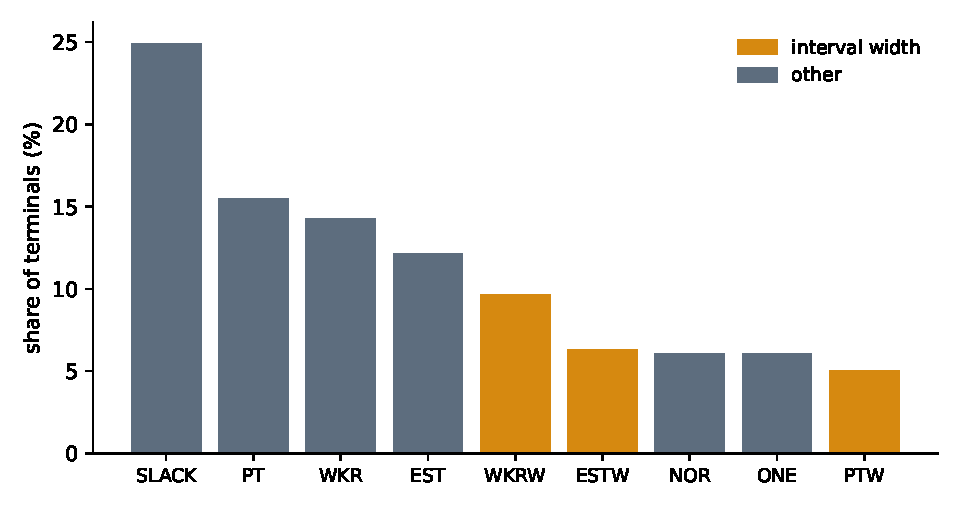
\includegraphics[width=.8\linewidth]{figures/fig_terminals.pdf}
\caption{Terminal usage across the 30 evolved rules, as a share of all
terminals. Interval-width terminals (amber) expose the magnitude of the
uncertainty to the rule.}
\label{fig:terminals}
\end{figure}

\subsection{Generalization to the full benchmark}
Table~\ref{tab:gp70} reports single-rollout $\RE$ per size class over all
70 instances, as mean $\pm$ standard deviation across the 30 evolved
rules and for the single best rule. The best rule attains $17.3\%$
global mean---evolved only on $20{\times}15$, its best class is the
unseen $50{\times}15$ ($13.3\%$), and the same pattern holds on
average ($13.5 \pm 1.4$). Because all terminals are per-operation
attributes with no size-bound quantities, transfer requires no
retraining or rescaling.

\begin{table}[t]
\centering\small
\caption{RE (\%) per size class, single deterministic rollout, over all
70 Taillard interval instances: mean $\pm$ sd across the 30 independently
evolved rules, and the best evolved rule.}
\label{tab:gp70}
\begin{tabular}{lccccccc|c}
\toprule
& $15{\times}15$ & $20{\times}15$ & $20{\times}20$ &
$30{\times}15$ & $30{\times}20$ & $50{\times}15$ & $50{\times}20$ & All \\
\midrule
Mean of 30 & $17.6{\pm}1.2$ & $17.5{\pm}1.2$ & $20.8{\pm}1.4$ &
$21.2{\pm}1.2$ & $25.2{\pm}1.2$ & $13.5{\pm}1.4$ & $15.0{\pm}1.2$ &
$18.7{\pm}0.8$ \\
Best rule & 16.6 & 15.3 & 17.9 & 18.9 & 24.6 & \textbf{13.3} & 14.4 &
\textbf{17.3} \\
\bottomrule
\end{tabular}
\end{table}

\subsection{The value of interval-awareness: terminal ablation}
\label{sec:ablation}
The interval-width terminals are the distinctive ingredient of this
setting, so we isolate their contribution. We re-run the full
evolution---30 independent seeds per configuration---with and without the
width terminals (\textit{PTW}, \textit{ESTW}, \textit{WKRW}) in the
terminal set, everything else held fixed, and compare the resulting
mean $\RE$ over the 70 instances with a paired Wilcoxon signed-rank test
on the shared seeds.
\todo{rellenar con la campaña 30$\times$3: media$\pm$std no-width vs full,
$\Delta$RE, y el estadístico de Wilcoxon. Redacción segun el signo del
efecto (paga / cotas de peor caso bastan).}

\subsection{Position among constructive methods}
All three constructive methods build one schedule per instance in a single
pass: MOR averages $45.5\%$ $\RE$, G\&T-MWKR $29.5\%$, and the evolved
rules $18.7 \pm 0.8$ on average ($17.3\%$ for the best rule).
The gap is not marginal and not an artefact of averaging: the best evolved
rule is better than \emph{both} baselines on every one of the $70$
instances, and a paired Wilcoxon signed-rank test rejects equality against
each baseline at $p<10^{-6}$ ($z=-7.3$). Per-instance figures are given in
Table~\ref{tab:perinstance} (appendix). Crucially, this quality comes at
no evaluation penalty over hand-crafted rules: evaluating the evolved
expression tree over the eligible set costs the same, within measurement
noise, as evaluating MOR or G\&T-MWKR (the three differ by under $15\%$ in
per-schedule construction time in our implementation), since all reduce to
one vectorized pass over eligible operations per decision. Both cost and
quality thus place the evolved rule with the constructive methods, orders
of magnitude below the search-based computational class in cost while
closing much of the quality gap to it. Figure~\ref{fig:ladder} places
these results on the full method ladder, including the published tabu
search~\cite{DiazTS2026} as the yardstick of the search-based class (an
iterative search of minutes per instance versus a single constructive
pass).

\begin{figure}[t]
\centering

\includegraphics[width=.85\linewidth]{figures/fig_ladder.pdf}
\caption{Constructive-method ladder on the 70 interval Taillard
instances. Bars are single-solution methods except where noted.}
\label{fig:ladder}
\end{figure}

\subsection{Sampling behaviour (GP-$\varepsilon$)}
Best-of-$N$ over all 70 instances (pools of $1024$
$\varepsilon$-randomized samples per instance): $18.6\%$ ($N{=}1$,
deterministic), $16.4\%$ ($16$), $14.9\%$ ($64$), $14.4\%$ ($256$),
$13.7\%$ ($1024$)---about $-4.9$ points over ten doublings
(Figure~\ref{fig:bestofn})---closing a substantial part of the gap to
population-based methods while remaining a set of independent constructive
passes, orders of magnitude below the iterative search in computational
class and trivially parallel.

\begin{figure}[t]
\centering
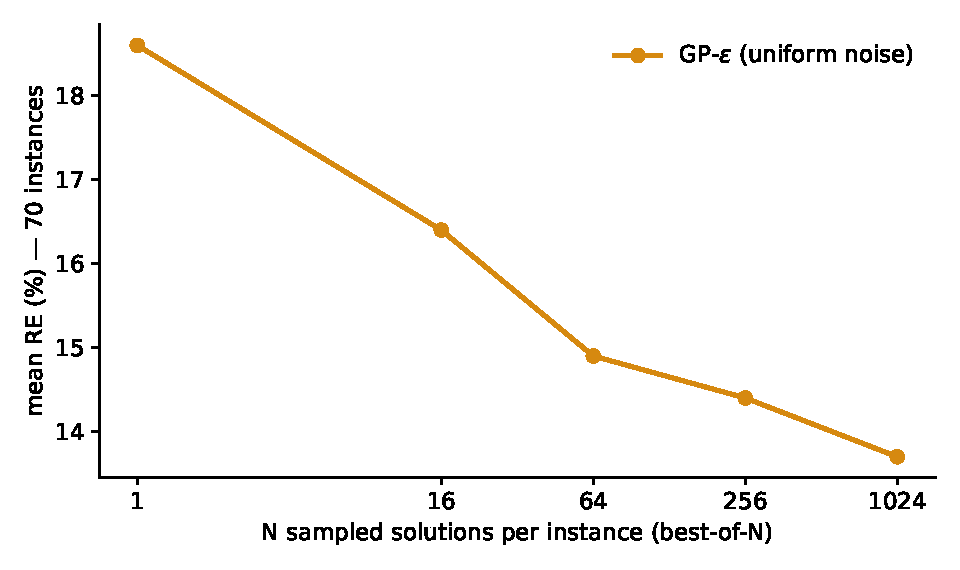
\includegraphics[width=.8\linewidth]{figures/fig_bestofN.pdf}
\caption{Best-of-$N$ curve of the evolved rule with uniform
$\varepsilon$-randomization ($\varepsilon{=}0.1$): mean RE over the 70
instances as the sampling budget doubles.}
\label{fig:bestofn}
\end{figure}

\subsection{Robustness under executional uncertainty}
\label{sec:robustness}
Relative error measures a-priori quality, but for the IJSP a schedule is
ultimately \emph{executed} under one realization of the durations. A good
predictive schedule is one whose executed makespan stays close to its
a-priori prediction. We quantify this with the $\bar\varepsilon$
robustness of~\cite{DiazGA2020}: for a schedule with fixed processing
order and predicted expected makespan $E[C_{\max}]$ (interval midpoint),
we draw $K{=}1000$ realizations of the durations (uniform on each
operation's interval), execute the fixed order, and average the relative
deviation of the executed makespan $C^{ex}_{\max}$ from the prediction,
$\bar\varepsilon = \frac1K\sum_k |C^{ex,k}_{\max}-E[C_{\max}]| /
E[C_{\max}]$. Lower is more robust. To probe behaviour under growing
uncertainty we also widen every interval symmetrically about its midpoint
by $+20\%$ and $+40\%$ (clipping negative bounds to zero), re-evaluating
the same processing orders.

The evolved rule does not merely produce lower-makespan schedules---it
produces \emph{more robust} ones, on two complementary measures
(Table~\ref{tab:robustness}). First, its predicted makespan interval is
the \emph{tightest}: a relative width of $12.6\%$ against $13.8\%$
(G\&T-MWKR) and $14.4\%$ (MOR), so the a-priori uncertainty attached to
the schedule is smaller. Second, and more tellingly, its executed
makespan tracks the prediction most closely: $\bar\varepsilon$ is lower
than for both baselines at the nominal width ($5.8$ versus $6.5$ for MOR
and $6.3$ for G\&T-MWKR), and its advantage \emph{widens} as uncertainty
grows (at $+40\%$: $7.7$ versus $8.9$ and $8.6$). Because the rule can
read interval widths, it favours dispatching decisions whose realized
outcome is less sensitive to how the durations materialize.
Figure~\ref{fig:robustness} shows the per-instance $\bar\varepsilon$
distributions.

\begin{table}[t]
\centering\small
\caption{Robustness over the 70 instances (lower is better on both
measures). \emph{Rel.\ width}: relative width of the predicted makespan
interval, $(\overline{C}_{\max}-\underline{C}_{\max})/E[C_{\max}]$ (\%).
$\bar\varepsilon$ ($\times10^3$): mean deviation of the executed makespan
from its prediction, at nominal interval widths and widened by $+20\%$ and
$+40\%$ (Monte Carlo, $K{=}1000$ realizations, common random numbers
across methods).}
\label{tab:robustness}
\begin{tabular}{lcccc}
\toprule
& & \multicolumn{3}{c}{$\bar\varepsilon$ ($\times10^3$)} \\
\cmidrule(l){3-5}
Method & Rel.\ width (\%) & $+0\%$ & $+20\%$ & $+40\%$ \\
\midrule
GP rule & \textbf{12.6} & \textbf{5.8} & \textbf{6.8} & \textbf{7.7} \\
G\&T-MWKR & 13.8 & 6.3 & 7.5 & 8.6 \\
MOR & 14.4 & 6.5 & 7.7 & 8.9 \\
\bottomrule
\end{tabular}
\end{table}

\begin{figure}[t]
\centering
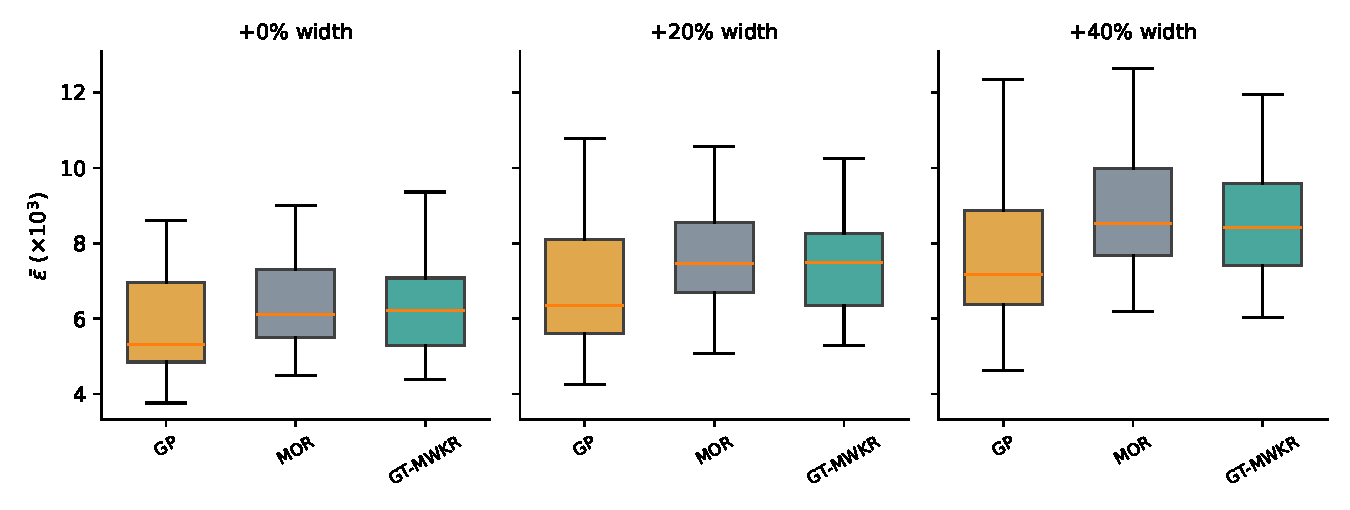
\includegraphics[width=\linewidth]{figures/fig_robustness_box.pdf}
\caption{Per-instance $\bar\varepsilon$ robustness by method at each
uncertainty level (lower is better). The evolved rule's robustness
advantage over the constructive baselines grows with interval width.}
\label{fig:robustness}
\end{figure}
\todo{tras la campaña: rehacer con la mejor regla de 30 semillas y anadir
el brazo no-width (robustez interval-aware vs ablacion); test estadistico.}

\subsection{Hyperparameter study}
\label{sec:tuning}
We tune the four qualitative knobs of the evolution (tournament size,
crossover probability, tree-size cap, elitism) with irace over a budget
of 200 experiments, each a full evolution (population $100$, $50$
generations) on the training instances evaluated on the development set,
with the conventional configuration seeded. The four elite
configurations agree on a higher selection pressure than the default
(tournament size $7$ versus $4$) and a crossover probability close to the
default ($0.72$--$0.77$ versus $0.8$); the tree-size cap, by contrast,
does not discriminate (surviving elites span caps of $20$, $30$ and
$40$), indicating the method is insensitive to bloat control within this
range. Throughout the race the statistical tests discard configurations
only weakly, itself evidence that performance is largely flat over the
hyperparameter space.

Under the same pre-registered confirmation applied to every design
decision---the winning configuration re-evolved over 30 independent
seeds and each resulting rule evaluated on all 70 instances---the tuned
configuration brings \emph{no} significant improvement: $18.99 \pm 1.33$
mean $\RE$ versus $18.68 \pm 0.84$ for the untuned default, with a paired
Wilcoxon signed-rank test on the shared seeds far from significance
($z=-0.96$); if anything, the stronger selection pressure increases
seed-to-seed variance. The one systematic effect of the tuned
configuration is \emph{structural}: with the same performance, it evolves
markedly smaller trees ($26.4$ versus $33.1$ nodes on average), i.e., the
tuning budget buys readability rather than quality. We therefore
characterize the method as robust to its evolutionary hyperparameters:
conventional settings are statistically indistinguishable from the irace
winner on unseen instances.

\section{Conclusions and Future Work}
\label{sec:conclusions}

We presented what is, to the best of our knowledge, the first GP
hyper-heuristic for job shop scheduling with interval durations, built on
a terminal set that exposes interval widths as first-class attributes.
The empirical conclusions are three. (i)~Evolved rules dominate every
deterministic constructive baseline on the 70-instance benchmark by a
wide, statistically significant margin ($18.7 \pm 0.8$ over 30
evolutions, $17.3\%$ for the best rule, versus $29.5\%$ for the
strongest baseline---which the best rule beats on all 70 instances) at
the cost of a single constructive pass, and (ii)~they
generalize zero-shot across all size
classes---evolved on $20{\times}15$, best on the unseen
$50{\times}15$---because the representation contains no size-bound
quantities. (iii)~The method is robust to its evolutionary
hyperparameters: a 200-experiment irace study confirmed over 30
evolutions per configuration yields no significant gain over
conventional settings, only systematically smaller trees at equal
performance.

Future work follows three lines. First, richer symbolic models:
ensembles of complementary rules~\cite{GilGala2021Ensembles} and
co-evolution of construction and tie-breaking. Second, using evolved rules as cheap, high-quality
population initializers for the metaheuristics that define the state of
the art in the IJSP, where preliminary pools built from randomized rule
rollouts are already compatible with the seeding protocol
of~\cite{DiazTS2026}. Third, a controlled comparison with learned
neural constructive policies under matched training and inference
budgets---the head-to-head evaluation that the recent
literature~\cite{Xu2025} identifies as missing.

\section*{Reproducibility}
The GP hyper-heuristic is implemented from scratch in pure Python/NumPy,
with no evolutionary-computation dependencies; evolved rules are stored
as plain JSON expression trees and evaluated as drop-in dispatching
strategies by the same environment used by every baseline.
\todo{URL/DOI del repositorio al publicar}

\appendix
\section{Per-instance results}
Table~\ref{tab:perinstance} lists, for each of the 70 interval Taillard
instances, the crisp lower bound and the single-pass $\RE$ (\%) of the
three deterministic constructive methods.

\begin{table}[t]
\centering\scriptsize
\caption{Per-instance $\RE$ (\%) of the constructive methods (single
deterministic pass). LB is the crisp Taillard lower bound.}
\label{tab:perinstance}
\setlength{\tabcolsep}{4pt}
\begin{tabular}{lrrrr@{\hskip 1.2em}lrrrr}
\toprule
Inst. & LB & MOR & G\&T & GP & Inst. & LB & MOR & G\&T & GP \\
\midrule
TA1 & 1231 & 29.7 & 26.1 & 18.6 & TA36 & 1819 & 57.4 & 42.8 & 20.0 \\
TA2 & 1244 & 34.8 & 27.8 & 15.5 & TA37 & 1771 & 43.0 & 35.6 & 23.4 \\
TA3 & 1218 & 42.9 & 33.2 & 16.1 & TA38 & 1673 & 50.6 & 28.0 & 21.1 \\
TA4 & 1175 & 62.6 & 27.7 & 17.0 & TA39 & 1795 & 50.2 & 28.9 & 18.7 \\
TA5 & 1224 & 50.7 & 33.0 & 8.8 & TA40 & 1651 & 42.7 & 42.3 & 21.5 \\
TA6 & 1238 & 36.6 & 18.2 & 16.7 & TA41 & 1906 & 53.5 & 45.0 & 32.3 \\
TA7 & 1227 & 39.4 & 26.1 & 21.8 & TA42 & 1884 & 61.3 & 38.1 & 23.0 \\
TA8 & 1217 & 41.3 & 25.0 & 13.9 & TA43 & 1809 & 61.4 & 39.8 & 24.2 \\
TA9 & 1274 & 38.2 & 28.2 & 17.9 & TA44 & 1948 & 58.8 & 34.7 & 24.4 \\
TA10 & 1241 & 38.0 & 22.1 & 19.6 & TA45 & 1997 & 59.5 & 33.7 & 16.2 \\
TA11 & 1357 & 49.9 & 30.7 & 16.5 & TA46 & 1957 & 59.7 & 31.6 & 24.5 \\
TA12 & 1367 & 47.8 & 34.6 & 15.4 & TA47 & 1807 & 78.3 & 30.0 & 23.2 \\
TA13 & 1342 & 46.5 & 26.9 & 14.9 & TA48 & 1912 & 52.2 & 33.7 & 26.3 \\
TA14 & 1345 & 44.1 & 29.7 & 9.7 & TA49 & 1931 & 46.9 & 35.3 & 22.8 \\
TA15 & 1339 & 51.3 & 30.6 & 16.4 & TA50 & 1833 & 56.2 & 46.2 & 29.7 \\
TA16 & 1360 & 35.8 & 34.0 & 18.5 & TA51 & 2760 & 38.2 & 34.7 & 26.3 \\
TA17 & 1462 & 50.1 & 17.7 & 12.8 & TA52 & 2756 & 38.1 & 26.5 & 10.5 \\
TA18 & 1377 & 54.2 & 31.8 & 18.0 & TA53 & 2717 & 28.2 & 18.3 & 11.0 \\
TA19 & 1332 & 43.2 & 29.3 & 13.7 & TA54 & 2839 & 23.6 & 16.1 & 4.7 \\
TA20 & 1348 & 43.7 & 24.1 & 16.9 & TA55 & 2679 & 37.6 & 29.2 & 13.9 \\
TA21 & 1642 & 40.8 & 28.0 & 15.4 & TA56 & 2781 & 44.8 & 19.8 & 10.9 \\
TA22 & 1561 & 46.3 & 30.8 & 24.6 & TA57 & 2943 & 29.9 & 20.0 & 12.7 \\
TA23 & 1518 & 45.2 & 35.3 & 22.5 & TA58 & 2885 & 30.5 & 26.3 & 13.7 \\
TA24 & 1644 & 36.2 & 23.8 & 14.4 & TA59 & 2655 & 45.2 & 28.2 & 19.0 \\
TA25 & 1558 & 53.2 & 33.8 & 17.4 & TA60 & 2723 & 25.3 & 19.8 & 10.1 \\
TA26 & 1591 & 52.4 & 31.2 & 18.0 & TA61 & 2868 & 48.7 & 25.4 & 17.2 \\
TA27 & 1652 & 49.8 & 31.1 & 16.9 & TA62 & 2869 & 43.5 & 27.6 & 14.9 \\
TA28 & 1603 & 38.8 & 26.8 & 17.7 & TA63 & 2755 & 46.0 & 23.8 & 11.8 \\
TA29 & 1583 & 56.4 & 32.0 & 12.3 & TA64 & 2702 & 43.3 & 28.4 & 11.5 \\
TA30 & 1528 & 53.3 & 36.1 & 19.8 & TA65 & 2725 & 44.7 & 30.0 & 19.7 \\
TA31 & 1764 & 34.4 & 34.4 & 15.2 & TA66 & 2845 & 38.1 & 28.0 & 14.8 \\
TA32 & 1774 & 55.7 & 33.3 & 21.2 & TA67 & 2825 & 58.4 & 26.1 & 12.7 \\
TA33 & 1788 & 41.6 & 34.8 & 22.7 & TA68 & 2784 & 45.8 & 19.1 & 10.3 \\
TA34 & 1828 & 34.8 & 31.8 & 16.4 & TA69 & 3071 & 38.0 & 22.8 & 11.4 \\
TA35 & 2007 & 30.5 & 24.1 & 9.2 & TA70 & 2995 & 52.3 & 23.4 & 20.2 \\
\bottomrule
\end{tabular}
\end{table}
\todo{tabla por instancia: se refresca con la mejor regla de la campana 30x3}

\begin{thebibliography}{10}

\bibitem{DiazGA2020}
H.~D\'iaz, I.~Gonz\'alez-Rodr\'iguez, J.~J.~Palacios, I.~D\'iaz,
C.~R.~Vela.
\newblock A genetic approach to the job shop scheduling problem with
  interval uncertainty.
\newblock In \textit{Information Processing and Management of Uncertainty
  in Knowledge-Based Systems (IPMU)}, pages 663--676. Springer, 2020.

\bibitem{DiazFEABC2023}
H.~D\'iaz, J.~J.~Palacios, I.~Gonz\'alez-Rodr\'iguez, C.~R.~Vela.
\newblock Fast elitist {ABC} for makespan optimisation in interval {JSP}.
\newblock \textit{Natural Computing}, 22(4):645--657, 2023.

\bibitem{DiazICAE2023}
H.~D\'iaz, J.~J.~Palacios, I.~Gonz\'alez-Rodr\'iguez, C.~R.~Vela.
\newblock An elitist seasonal artificial bee colony algorithm for the
  interval job shop.
\newblock \textit{Integrated Computer-Aided Engineering}, 30(3):223--242, 2023.

\bibitem{DiazTS2026}
H.~D\'iaz et al.
\newblock Neighbourhood structures and ranking operators for the interval
  job shop scheduling problem.
\newblock Under review, 2026.

\bibitem{Lei2012}
D.~Lei.
\newblock Population-based neighborhood search for job shop scheduling
  with interval processing time.
\newblock \textit{Computers \& Industrial Engineering}, 62(4):1200--1208,
  2012.

\bibitem{Branke2016}
J.~Branke, S.~Nguyen, C.~W.~Pickardt, M.~Zhang.
\newblock Automated design of production scheduling heuristics: a review.
\newblock \textit{IEEE Transactions on Evolutionary Computation},
  20(1):110--124, 2016.

\bibitem{Nguyen2017}
S.~Nguyen, Y.~Mei, M.~Zhang.
\newblock Genetic programming for production scheduling: a survey with a
  unified framework.
\newblock \textit{Complex \& Intelligent Systems}, 3(1):41--66, 2017.

\bibitem{Karunakaran2017}
D.~Karunakaran, Y.~Mei, G.~Chen, M.~Zhang.
\newblock Dynamic job shop scheduling under uncertainty using genetic
  programming.
\newblock In \textit{Intelligent and Evolutionary Systems}, pages
  195--210. Springer, 2017.

\bibitem{Xu2025}
M.~Xu, Y.~Mei, F.~Zhang, M.~Zhang.
\newblock Learn to optimise for job shop scheduling: a survey with
  comparison between genetic programming and reinforcement learning.
\newblock \textit{Artificial Intelligence Review}, 58:160, 2025.

\bibitem{GilGala2021Ensembles}
F.~J.~Gil-Gala, C.~Menc\'ia, M.~R.~Sierra, R.~Varela.
\newblock Learning ensembles of priority rules for online scheduling by
  hybrid evolutionary algorithms.
\newblock \textit{Integrated Computer-Aided Engineering}, 28(1):65--80,
  2021.

\bibitem{GilGala2025SSHE}
F.~J.~Gil-Gala, M.~\DJ ura\v{s}evi\'c, M.~R.~Sierra, R.~Varela.
\newblock Tree search hyper-heuristic with application to combinatorial
  optimization.
\newblock \textit{Journal of Heuristics}, 31:25, 2025.

\bibitem{GilGala2025GRASB}
F.~J.~Gil-Gala, M.~\DJ ura\v{s}evi\'c, M.~R.~Sierra, J.~Puente.
\newblock Greedy randomised adaptive solution builder using priority
  rules.
\newblock In \textit{Proc. Genetic and Evolutionary Computation Conference
  Companion (GECCO '25)}, pages 211--214. ACM, 2025.

\bibitem{Zhang2020L2D}
C.~Zhang, W.~Song, Z.~Cao, J.~Zhang, P.~S.~Tan, C.~Xu.
\newblock Learning to dispatch for job shop scheduling via deep
  reinforcement learning.
\newblock \textit{NeurIPS}, 2020.

\bibitem{Park2021GNN}
J.~Park, J.~Chun, S.~H.~Kim, Y.~Kim, J.~Park.
\newblock Learning to schedule job-shop problems: representation and
  policy learning using graph neural network and reinforcement learning.
\newblock \textit{International Journal of Production Research},
  59(11):3360--3377, 2021.

\bibitem{FuzzyJSPRef}
J.~J.~Palacios, I.~Gonz\'alez-Rodr\'iguez, C.~R.~Vela, J.~Puente.
\newblock Coevolutionary makespan optimisation through different ranking
  methods for the fuzzy flexible job shop.
\newblock \textit{Fuzzy Sets and Systems}, 278:81--97, 2015.

\end{thebibliography}

\end{document}
